% !TeX root = ../main.tex
% Add the above to each chapter to make compiling the PDF easier in some editors.

\begin{figure} [h!]
	\centering
	\begin{subfigure}[t]{1.0\textwidth}
		\centering
		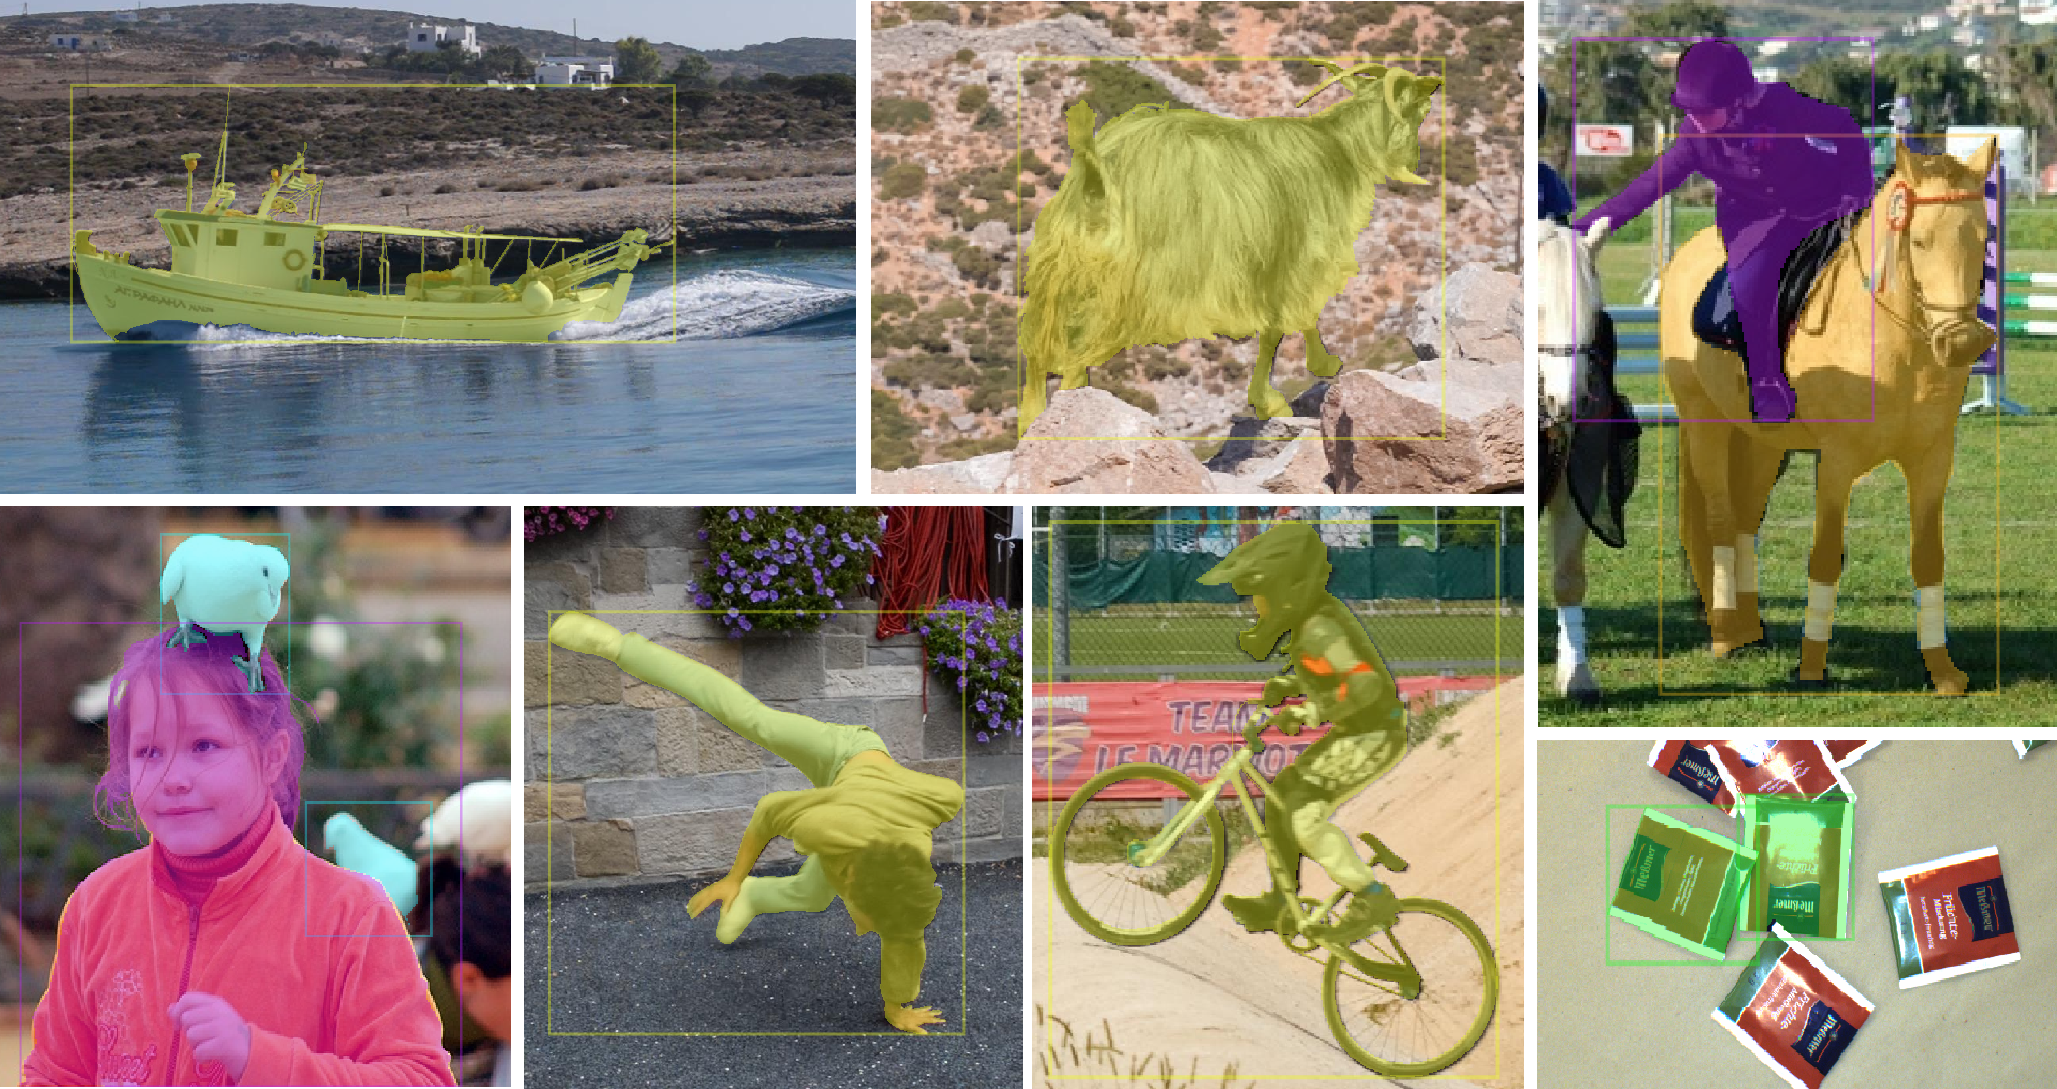
\includegraphics[width=\textwidth]{figures/appendix/benchmark_dataset_examples/standard_collage.png}
		\caption{
			Presentation of benchmark images from the domain $ standard $.
		}\label{fig:appendix_domain_standard}
	\end{subfigure}
	\\
	\begin{subfigure}[t]{1.0\textwidth}
		\centering
		\includegraphics[width=\textwidth]{figures/appendix/benchmark_dataset_examples/urban_collage.png}
		\caption{
			Presentation of benchmark images from the domain $ urban $.			
		} \label{fig:appendix_domain_urban}
	\end{subfigure}
	\caption[Illustration of various benchmark images]{	
		Presentation of benchmark images from the four domain $ standard $, $ urban $, $ industrial $, and $ anomaly $.	
		Only the objects that should be labeled are shown with their object mask.
	}\label{fig:appendix_benchmark_domains}
\end{figure}

\begin{figure} \ContinuedFloat
	\begin{subfigure}[t]{1.0\textwidth} 
		\centering
		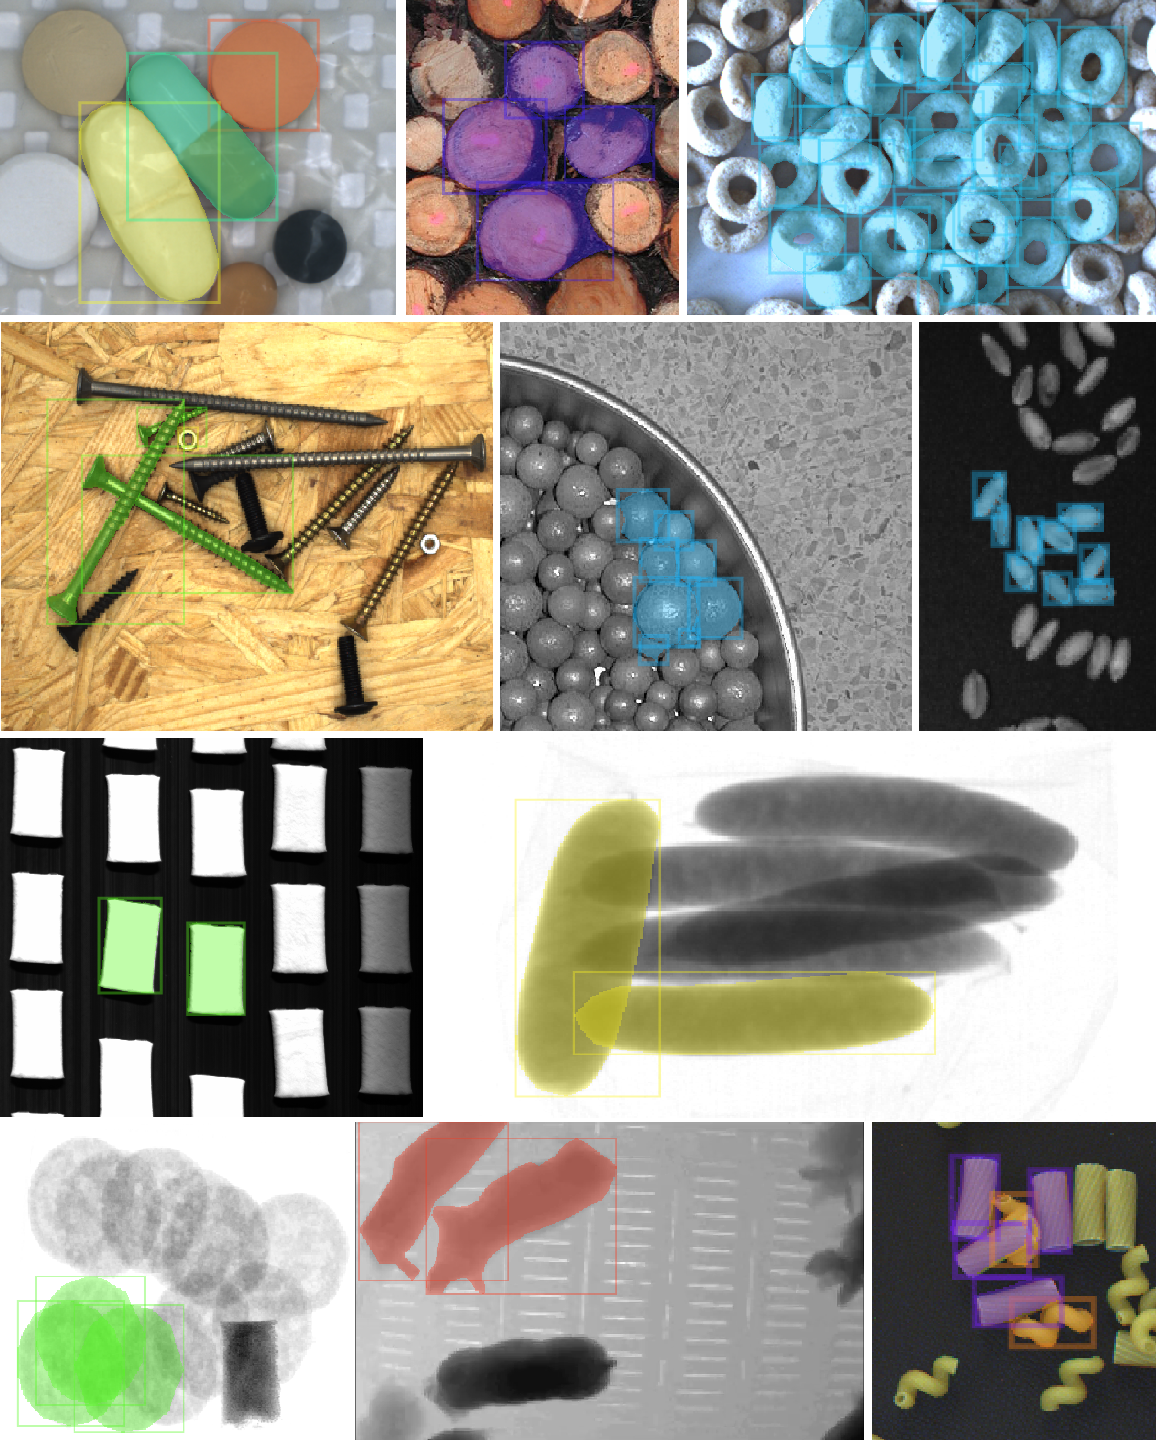
\includegraphics[width=\textwidth]{figures/appendix/benchmark_dataset_examples/industrial_collage.png}
		\caption{
			Presentation of benchmark images from the domain $ industrial $.
			In the images, that contain a lot of objects with masks only a limited part should be labeled.		
			In some illustrations only a small section is shown, to better present the small objects.
		} \label{fig:appendix_domain_industrial}
	\end{subfigure}
\end{figure}
% TODO add more example for industrial
	
\begin{figure} \ContinuedFloat
	\begin{subfigure}[t]{1.0\textwidth} 
		\centering
		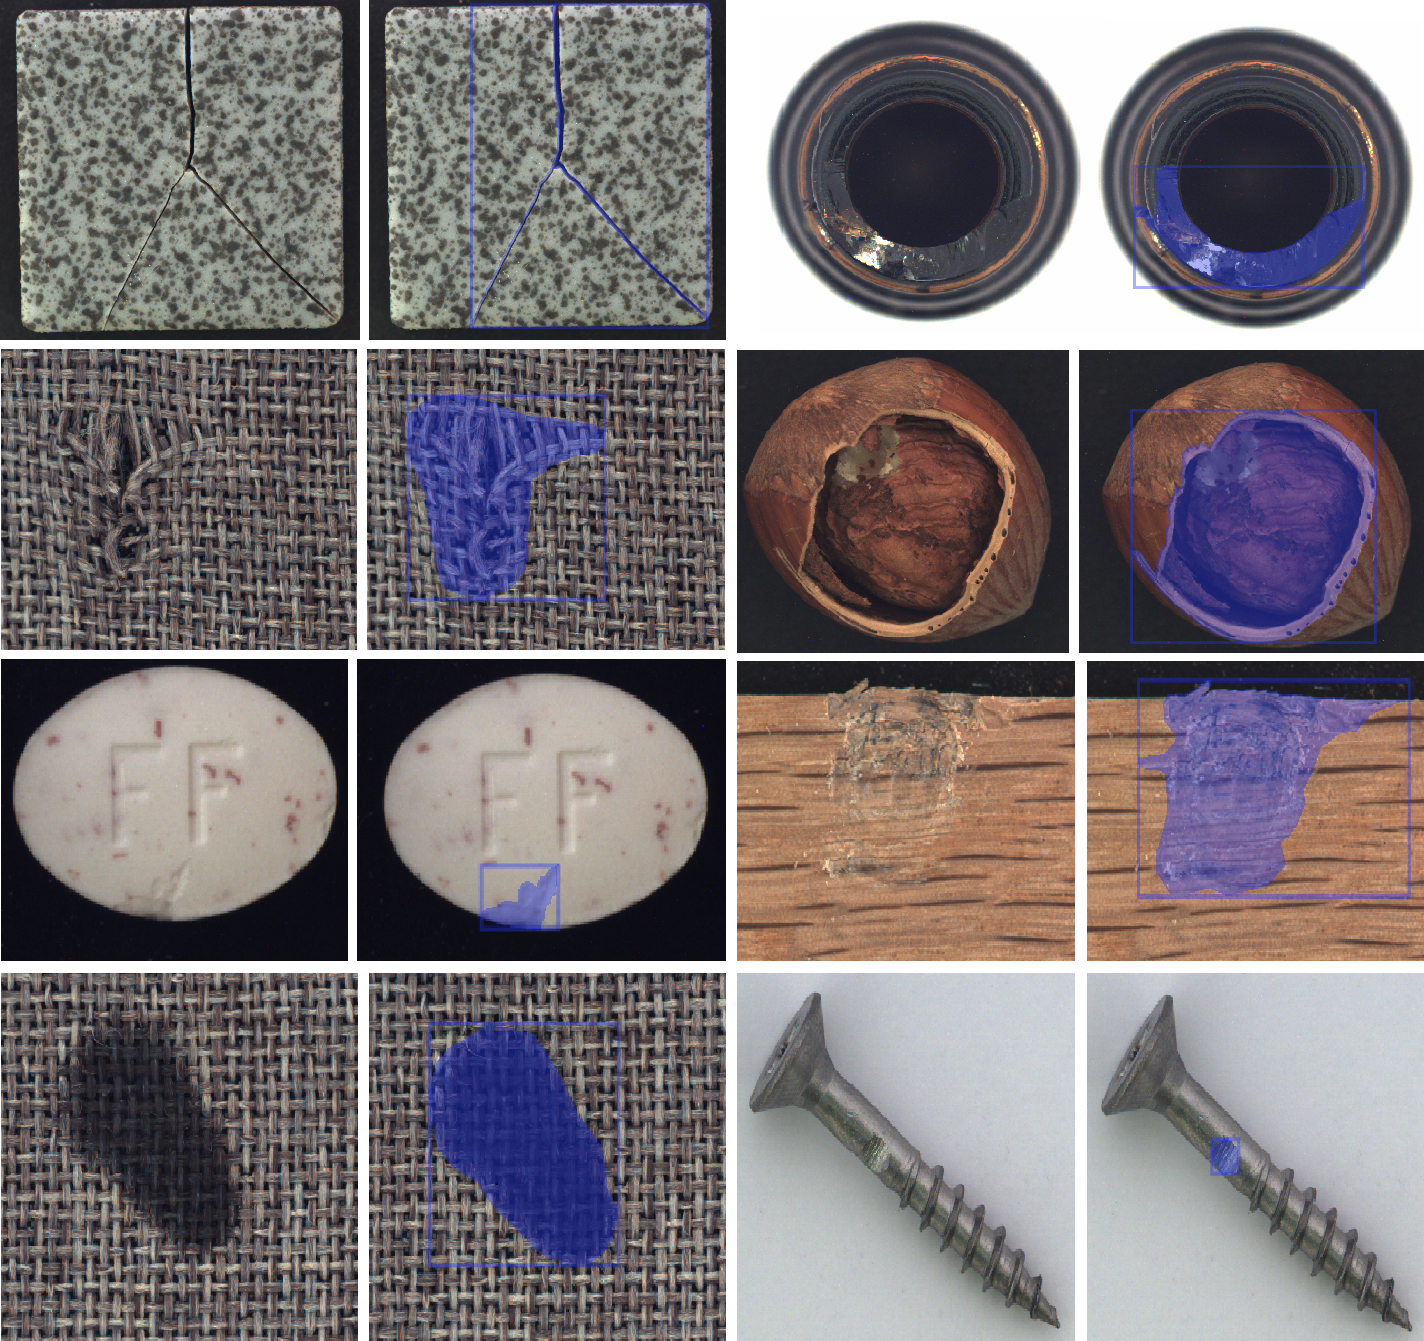
\includegraphics[width=\textwidth]{figures/appendix/benchmark_dataset_anomaly_examples/anomaly_collage.png}
		\caption{
			Presentation of benchmark images from the domain $ anomaly $.
			In order to make the error clearly visible, the image was displayed once with and once without the object mask, which is above the anomaly.
			The images with such anomalies mostly origin from industrial contexts with the aim of detecting errors.			
		} \label{fig:appendix_domain_anomaly}
	\end{subfigure}
\end{figure}